\documentclass{article}
\usepackage{graphicx}
\usepackage[margin=1.5cm]{geometry}
\usepackage{amsmath}

\begin{document}
\twocolumn

\title{Warm Up: Unit 0: Energy, Work, Food, and Polar Travel}
\author{Prof. Jordan C. Hanson}

\maketitle

\section{Memory Bank}
\begin{itemize}
\item 1 Joule = 1 Newton $\times$ 1 meter
\item 1 calorie = 4.184 Joules
\item 1 kcal = 4184 Joules
\item Carbohydrates: 4 kcal/gram
\item Protein: 4 kcal/gram
\item Fat: 9 kcal/gram
\item 1 kilogram = 1000 grams
\item 1 Watt = 1 Joule / 1 second
\item A Watt is a unit of \textit{power}, while a Joule is a unit of \textit{energy.}
\end{itemize}

\section{Work and Energy}

\begin{enumerate}
\item Convert the following:
\begin{itemize}
\item 440 Joules to calories.
\item 2500 calories to kcal.
\item $2.5 \times 10^6$ Joules to kcal.
\end{itemize} \vspace{2cm}
\item (a) If an activity requires $2.5 \times 10^6$ Joules to complete, and it needs to be done in 6 hours, how many Watts of power does this imply? (b) How many Joules of energy are required for playing tennis for 3 hours? \\ \vspace{3cm}
\item (a) Convert your response for part (b) of the previous exercise to kcal.  (b) How many grams of carbohydrates would provide this energy?
\end{enumerate}

\begin{figure}
\centering
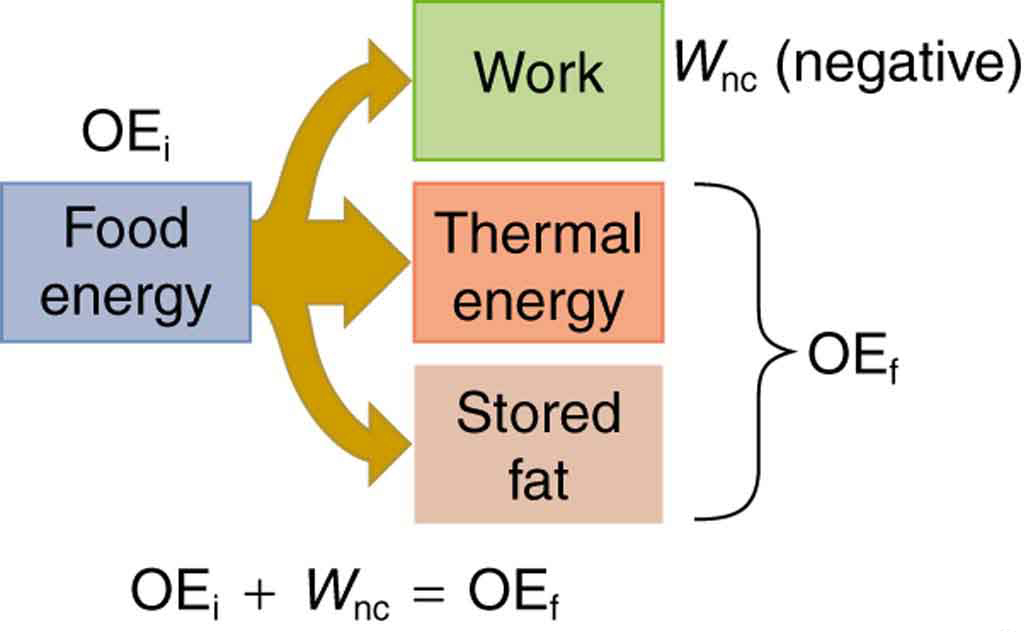
\includegraphics[width=0.33\textwidth]{figures/work1.jpeg} \\ \vspace{1cm}
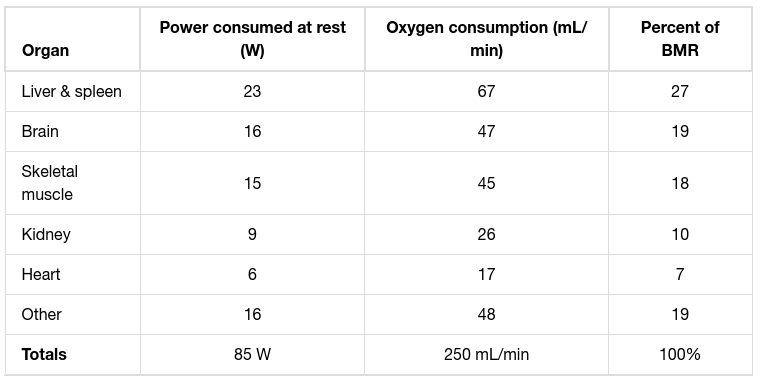
\includegraphics[width=0.5\textwidth]{figures/work2.png} \\ \vspace{1cm}
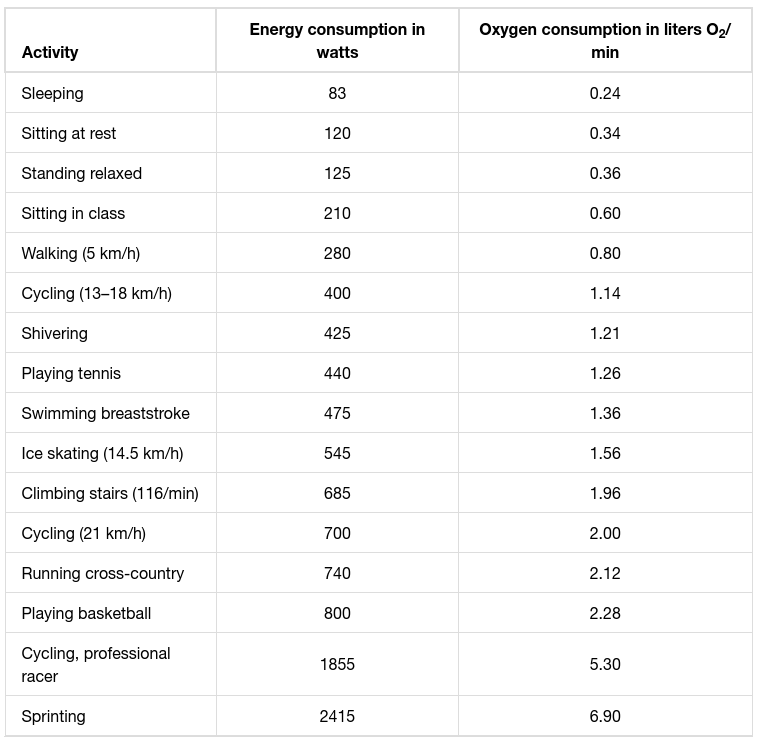
\includegraphics[width=0.5\textwidth]{figures/work3.png}\\ \vspace{1cm}
\end{figure}

\end{document}
